\documentclass[8pt, a4paper, notitlepage]{extreport}
\usepackage{kactlpkg}
\kactlcontentdir{content}
\usepackage{amssymb}
\usepackage{amsmath}

\university{NRU HSE (Mikhnenko, Novikov, Stepanov)}{National Research University Higher School of Economics}{hse}
\team{Surstrumien Bobra}{Alexey Mikhnenko, Vladimir Novikov, Anton Stepanov}
% \contest{ICPC World Finals 2025}{?????, 2025}
\contest{\ }{\today}
% \enablecolors

% \renewcommand*\contentsname{Algo}

\begin{document}
	\maketeampage
	% Small KACTL header on the first page:
	% \maketitle{``One Last Time'' Edition}{\today}
	
	\begin{multicols*}{3}
	
	\thispagestyle{fancy}
	% Table of contents, without subsections:
	\setcounter{tocdepth}{0}

	% \tableofcontents

	% \kactlchapter{contest}
	% \kactlchapter{data-structures}
	% \kactlchapter{numerical}
	% \kactlchapter{number-theory}
	% \kactlchapter{combinatorial}
	% \kactlchapter{graph}
	% \kactlchapter{geometry}
	
	% \kactlchapter{various}

	\kactlchapter{contest}
	% \columnbreak
	\kactlchapter{cpp}
	% \columnbreak
	\kactlchapter{strings}
	% \columnbreak
	\kactlchapter{graph}
	% \columnbreak
	\kactlchapter{geometry}
	% \columnbreak
	\kactlchapter{math}
	%\columnbreak
	%\kactlchapter{integrals}
	\end{multicols*}
	\begin{multicols*}{3}
	\kactlchapter{integrals}
	\end{multicols*}

	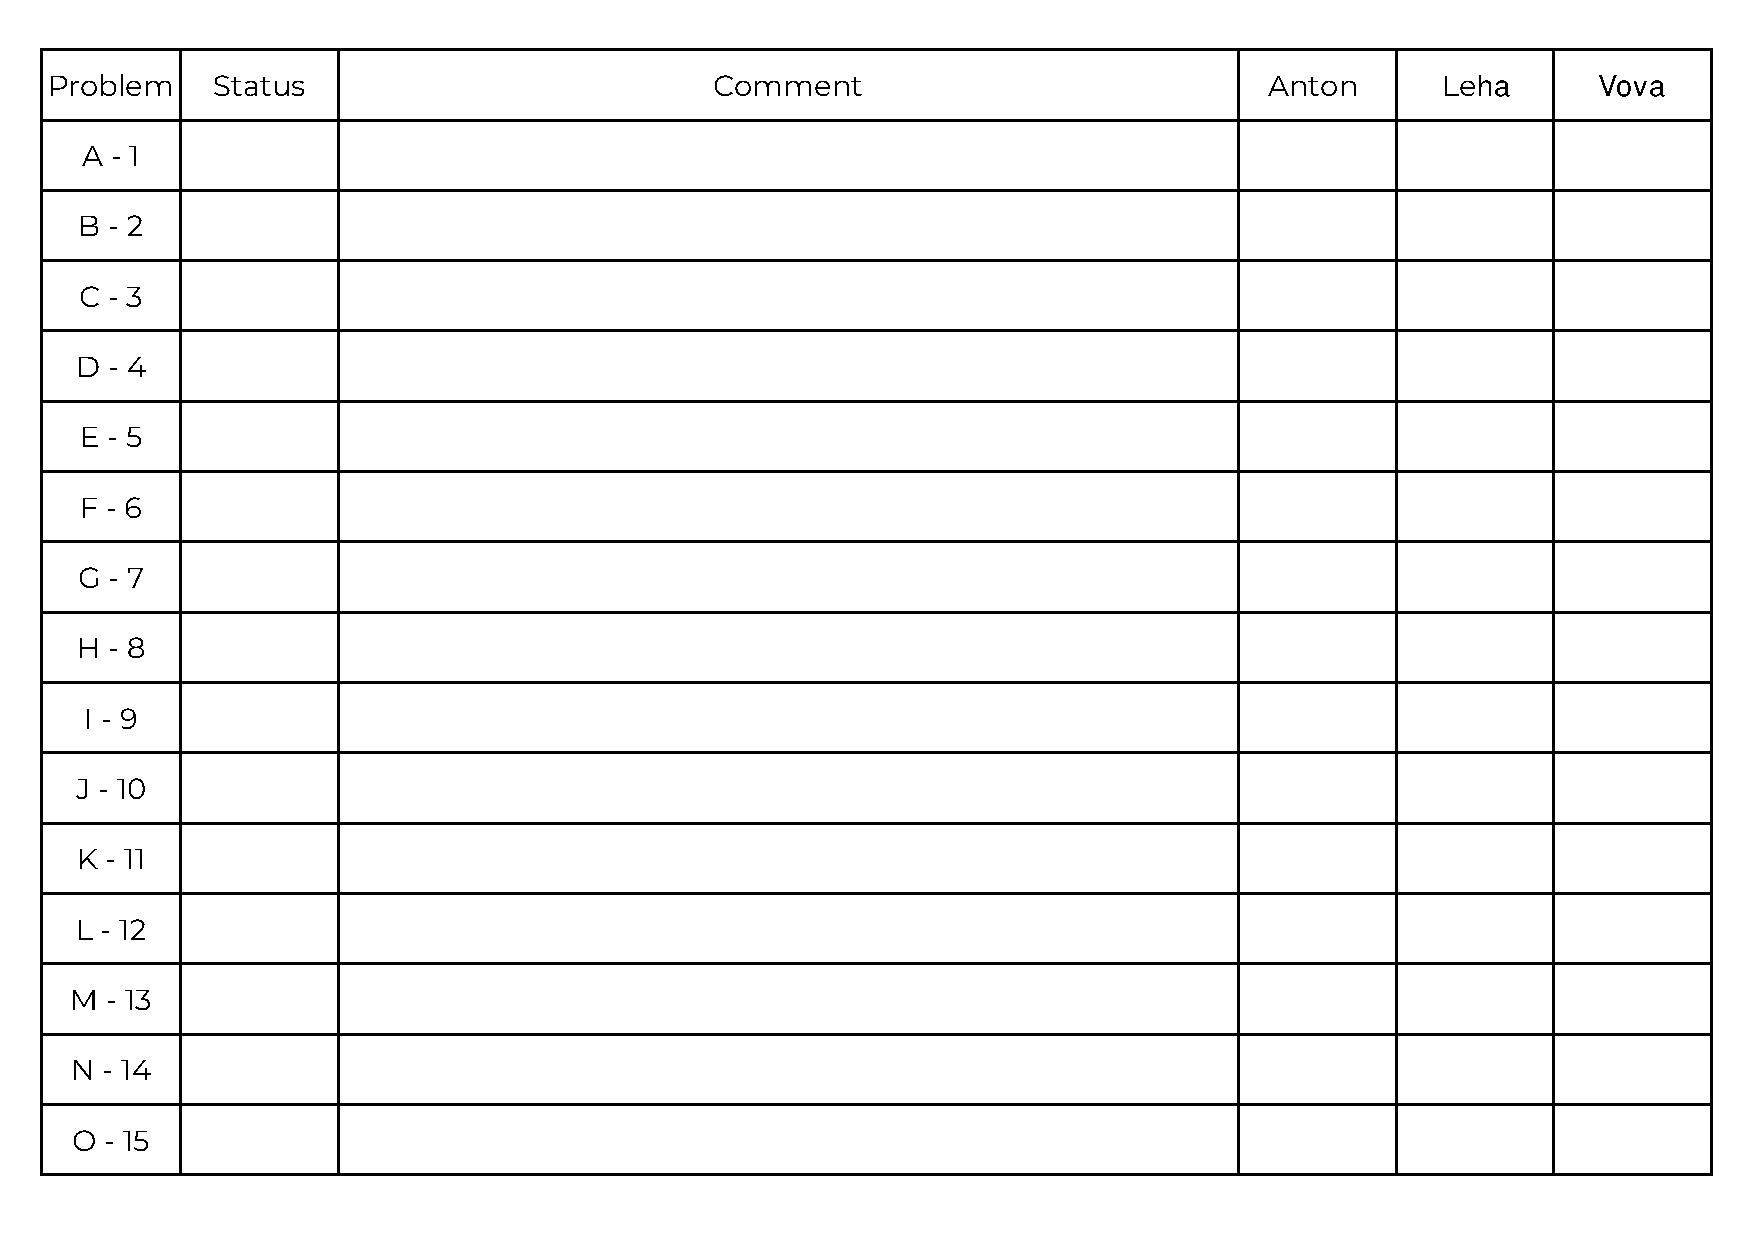
\includepdf[pages=-]{content/contest/SurstrumienBobraMonitor.pdf}

	% \begin{multicols*}{2}
	% \kactlchapter{appendix}
	% \end{multicols*}
\end{document}
